% Copyright 2020  Ed Bueler

\documentclass[10pt,hyperref]{beamer}

\mode<presentation>{
  \usetheme{Madrid}
  \usecolortheme{beaver}
  \setbeamercovered{transparent}  
  \setbeamerfont{frametitle}{size=\large}
}

\setbeamercolor*{block title}{bg=red!10}
\setbeamercolor*{block body}{bg=red!5}

\usepackage[english]{babel}
\usepackage[latin1]{inputenc}
\usepackage{times}
\usepackage[T1]{fontenc}
% Or whatever. Note that the encoding and the font should match. If T1
% does not look nice, try deleting the line with the fontenc.

\usepackage{empheq}
\usepackage{xspace}
\usepackage{verbatim,fancyvrb}

\usepackage{tikz}
\usetikzlibrary{shapes,arrows.meta,decorations.markings,decorations.pathreplacing,fadings,positioning}

\usepackage{hyperref}

% If you wish to uncover everything in a step-wise fashion, uncomment
% the following command: 
%\beamerdefaultoverlayspecification{<+->}

\newcommand{\ba}{\mathbf{a}}
\newcommand{\bb}{\mathbf{b}}
\newcommand{\bc}{\mathbf{c}}
\newcommand{\bg}{\mathbf{g}}
\newcommand{\bq}{\mathbf{q}}
\newcommand{\br}{\mathbf{r}}
\newcommand{\bx}{\mathbf{x}}
\newcommand{\by}{\mathbf{y}}
\newcommand{\bv}{\mathbf{v}}
\newcommand{\bu}{\mathbf{u}}
\newcommand{\bw}{\mathbf{w}}

\newcommand{\bF}{\mathbf{F}}

\newcommand{\grad}{\nabla}
\newcommand{\Div}{\nabla\cdot}

\newcommand{\CC}{\mathbb{C}}
\newcommand{\RR}{\mathbb{R}}

\newcommand{\ddt}[1]{\ensuremath{\frac{\partial #1}{\partial t}}}
\newcommand{\ddx}[1]{\ensuremath{\frac{\partial #1}{\partial x}}}
\newcommand{\Matlab}{\textsc{Matlab}\xspace}
\newcommand{\Octave}{\textsc{Octave}\xspace}
\newcommand{\eps}{\epsilon}

\newcommand{\ip}[2]{\left<#1,#2\right>}

\newcommand{\trefcolumn}[1]{\begin{bmatrix} \phantom{x} \\ #1 \\ \phantom{x} \end{bmatrix}}
\newcommand{\trefmatrixtwo}[2]{\left[\begin{array}{c|c|c} & & \\ #1 & \dots & #2 \\ & & \end{array}\right]}
\newcommand{\trefmatrixthree}[3]{\left[\begin{array}{c|c|c|c} & & & \\ #1 & #2 & \dots & #3 \\ & & & \end{array}\right]}
\newcommand{\trefmatrixgroups}[4]{\left[\begin{array}{c|c|c|c|c|c} & & & & & \\ #1 & \dots & #2 & #3 & \dots & #4 \\ & & & & & \end{array}\right]}

\newcommand{\blocktwo}[4]{\left[\begin{array}{c|c} #1 & #2 \\ \hline #3 & #4 \end{array}\right]}

\newcommand{\bqed}{{\color{blue}\qed}}
\newcommand{\ds}{\displaystyle}

\newcommand\mynum[1]{{\renewcommand{\insertenumlabel}{#1}%
      \usebeamertemplate{enumerate item} \,}}


\AtBeginSection[]
{
  \begin{frame}<beamer>
    \frametitle{Outline}
    \tableofcontents[currentsection,hideallsubsections]
  \end{frame}
}

\title[Finite volume methods]{Finite volume methods for \\ advection equations and hyperbolic systems}

%\subtitle{part I: xx}

\author{Ed Bueler}

\institute[UAF]{University of Alaska Fairbanks}

\date{June 2020}


\begin{document}
\beamertemplatenavigationsymbolsempty

\begin{frame}
  \maketitle
\end{frame}

\begin{frame}
  \frametitle{Outline}
  \tableofcontents[hideallsubsections]
\end{frame}


\begin{frame}[fragile]
\frametitle{overview}

\begin{itemize}
\item numerical solutions of first-order PDEs
    \begin{itemize}
    \item[$\circ$] finite volume (FV) methods
    \item[$\circ$] genuine introduction
    \end{itemize}
\item we will solve these hyperbolic equations:

\bigskip
\begin{center}
\begin{tikzpicture}[scale=0.9,
                    >={Latex[length=2mm]},
  eqn/.style={
     rectangle,draw,fill=white,align=center,line width=0.6pt,minimum width=15mm}]

%center
\draw[line width=1pt] (0,0)     node[eqn] (scalaradvect)  {\mynum{1}\&\mynum{2} scalar advection \\ {\Large \strut} $u_t + a u_x=0$};
\draw[line width=1pt] (3,-1.7)     node[eqn] (scalartwod)  {\mynum{4} scalar advection in 2D \\ {\Large \strut} $u_t + a u_x + b u_y=0$};
\draw[line width=1pt] (-2,-1.7)    node[eqn] (linearsystem)  {\mynum{3} linear system \\ {\Large \strut} $\bq_t + A\, \bq_x=0$};
\draw[line width=1pt] (-2,-3.55)    node[eqn] (generalsystem)  {\mynum{5} conservation-law system \\ {\Large \strut} $\bq_t + \bF(t,x,\bq)_x=\bg(t,x,\bq)$};

\path[-Latex]
   ([xshift=-2em]scalaradvect.south) edge node {} (linearsystem)
   ([xshift=2em]scalaradvect.south) edge node {} (scalartwod)
   (linearsystem.south) edge node {} (generalsystem);
\end{tikzpicture}

\bigskip
    \begin{itemize}
    \item[$\circ$] ``hyperbolic'' means finite speed of influence
    \item[$\circ$] arrows show generalizations
    \end{itemize}
\end{center}
\end{itemize}
\end{frame}


\begin{frame}{references}
\begin{itemize}
\item \alert{R.~J.~LeVeque, \emph{Finite Volume Methods for Hyperbolic Problems}, Cambridge University Press, 2002}

\bigskip
\item \small K.~W.~Morton and D.~F.~Mayers, \emph{Numerical Solutions of Partial Differential Equations: An Introduction}, Cambridge University Press, 2nd ed., 2005
\item \small W.~Hundsdorfer and J.~G.~Verwer, \emph{Numerical Solution of Time-Dependent Advection-Diffusion-Reaction Equations}, Springer, 2003  \, \mynum{2}
\item \small E.~Bueler, \emph{PETSc for Partial Differential Equations}, SIAM Press, 2020?  \, \mynum{4}
\end{itemize}
\end{frame}


\begin{frame}{visual example 1: exact and numerical solutions}

\begin{itemize}
\item $u_t + 2 u_x = 0$, $u(t,x)$, $u(t,0)=0$ SHOW exact solution and Lax-Wendroff
\end{itemize}
\end{frame}


\begin{frame}{visual example 2: merely a numerical solution}

\begin{itemize}
\item SHOW numerical solution of shallow water
\end{itemize}
\end{frame}



\section{scalar advection equation}

\begin{frame}{solution by characteristics}

\begin{itemize}
\item the \emph{scalar advection equation}:
    $$u_t + a u_x=0$$
    \begin{itemize}
    \item[$\circ$] we will only need $a\in\RR$ constant in this part, so let's assume that
    \end{itemize}
\item x
\end{itemize}
\end{frame}


\begin{frame}{upwind and Lax-Wendroff schemes}

\begin{itemize}
\item upwind if $a>0$
    $$\frac{u_j^{n+1} - u_j^n}{\Delta t} + a \frac{u_j^n - u_{j-1}^n}{\Delta t} = 0$$
\item Lax-Wendroff if $a$ FIXME
    $$\frac{u_j^{n+1} - u_j^n}{\Delta t} + a \frac{u_j^n - u_{j-1}^n}{\Delta t} = 0$$
\end{itemize}
\end{frame}


\begin{frame}{results}

\begin{itemize}
\item results from short \Matlab code\footnote{\href{http://bueler.github.io/codes/adcompare.m}{\texttt{bueler.github.io/codes/adcompare.m}}}
\end{itemize}
\end{frame}


\begin{frame}{method-of-lines thinking (MOL)}

\begin{itemize}
\item x
\end{itemize}
\end{frame}


\begin{frame}{x}

\begin{itemize}
\item x
\end{itemize}
\end{frame}


\begin{frame}{x}

\begin{itemize}
\item x
\end{itemize}
\end{frame}


\section{high-resolution methods}

\begin{frame}{Godunov's barrier theorem}

\begin{itemize}
\item can we do better?
\end{itemize}

\begin{theorem}[\emph{Godunov's barrier theorem, 1959}]  A monotonicity-preserving linear scheme for the 1D constant-coefficient equation $u_t + \alpha u_x=0$ cannot have second-order (or higher) local truncation error in $x$.\end{theorem}
\end{frame}

\begin{frame}{x}

\begin{itemize}
\item x
\end{itemize}
\end{frame}


\section{linear systems}

\begin{frame}{linear systems}

\begin{itemize}
\item system for $\bq(t,x) \in \RR^n$ with $A\in\RR^{n\times n}$ constant:
  $$\bq_t + A\, \bq_x=0$$
\item for example,
    \begin{itemize}
    \item[$\circ$] \emph{acoustics} (and classic wave equation)
        $$\bq = \begin{bmatrix} p \\ u \end{bmatrix}, \,\, A = \begin{bmatrix} 0 & K_0 \\ \frac{1}{\rho_0} & 0 \end{bmatrix} \quad \implies \quad \begin{matrix} p_t + K_0 u_x = 0 \\ u_t + \frac{1}{\rho_0} p_x = 0 \end{matrix} \qquad \begin{pmatrix} \, {\large \strut} p_{tt} = \frac{K_0}{\rho_0} p_{xx}\, \\ \, {\large \strut} u_{tt} = \frac{K_0}{\rho_0} u_{xx}\, \end{pmatrix}$$
    \item[$\circ$] \underline{linearized} \emph{shallow water equations}
        $$\bq = \begin{bmatrix} h \\ h u \end{bmatrix}, \,\, A = \begin{bmatrix} 0 & 1 \\ -u_0^2+gh_0 & 2 u_0 \end{bmatrix} \, \implies \, {\footnotesize \begin{matrix} {\large \strut} h_t + (hu)_x = 0 \\ {\large \strut} (h u)_t + (-u_0^2+gh_0) h_x + 2u_0 (h u)_x = 0 \end{matrix} }$$
    \item[$\circ$] boringly decoupled
        $$\bq = \begin{bmatrix} u \\ v \\ w \end{bmatrix}, \,\, A = \begin{bmatrix} a & 0 & 0 \\ 0 & b & 0 \\ 0 & 0 & c \end{bmatrix} \, \implies \begin{matrix} u_t + a u_x = 0 \\ v_t + b v_x = 0 \\ w_t + c w_x = 0 \end{matrix}$$
    \end{itemize}
\end{itemize}
\end{frame}


\begin{frame}{eigenvectors decouple systems}

\begin{itemize}
\item the system $\bq_t + A\, \bq_x=0$ is \emph{hyperbolic} if $A$ is diagonalizable and all of the eigenvalues of $A$ are real
    \begin{itemize}
    \item[$\circ$] diagonalizable means there are eigenvectors of $A$ which form a basis of $\RR^n$
    \end{itemize}
\item consider \emph{left eigenvectors} of $A$, namely vectors $\bw_k \in \RR^n$ so that
    $$\bw_k^\top A = \lambda_k \bw_k^\top$$

\vspace{-2mm}
    \begin{itemize}
    \item[$\circ$] $\lambda_k$ are \emph{eigenvalues}, real numbers if system is hyperbolic
    \item[$\circ$] $\bw$ are column vectors so $\bw_k^\top$ are row vectors
    \end{itemize}
\item decouple the system $\bq_t + A\, \bq_x=0$ by multiplying by $\bw_k^\top$:
\begin{align*}
\bw_k^\top \bq_t + \bw_k^\top A\, \bq_x &= 0 \\
\bw_k^\top \bq_t + \lambda_k \bw_k^\top \bq_x &= 0 \\
(v_k)_t + \lambda_k (v_k)_x &= 0
\end{align*}
\item scalar functions $v_k(t,x) = \bw_k^\top \bq(t,x)$ satisfy decoupled advection eqns:
   $$(v_k)_t + \lambda_k (v_k)_x = 0$$
\end{itemize}
\end{frame}


\begin{frame}{inner products, left eigenvectors, transposes, and \Matlab}

\begin{itemize}
\item $\bu^\top \bv = \ip{\bu}{\bv}$
\item same as right for $A^\top$
\item basis of left iff basis of right
\item in \Matlab, find left this way
\end{itemize}
\end{frame}


\begin{frame}{Riemann solver}

\begin{itemize}
\item x
\end{itemize}
\end{frame}


\begin{frame}{two ways of thinking}

\begin{itemize}
\item Riemann solver at cell face $(t,x_{j+1/2})$ versus characteristic to $(t_{n+1},x_j)$
\end{itemize}
\end{frame}

\section{scalar advection in 2D}

\begin{frame}{x}

\begin{itemize}
\item using C using PETSc \dots not shown \dots see \,\href{https://github.com/bueler/p4pdes}{\texttt{github.com/bueler/p4pdes}}
\item x
\end{itemize}
\end{frame}


\section{nonlinear conservation-law systems}

\begin{frame}{x}

\begin{itemize}
\item x
\end{itemize}
\end{frame}


\begin{frame}{x}

\begin{itemize}
\item x
\end{itemize}
\end{frame}


\begin{frame}[fragile]
\frametitle{xx}

\begin{itemize}
\item xx:

\medskip
\begin{Verbatim}[fontsize=\scriptsize]
>> size(A)
ans =
      201        5
\end{Verbatim}

%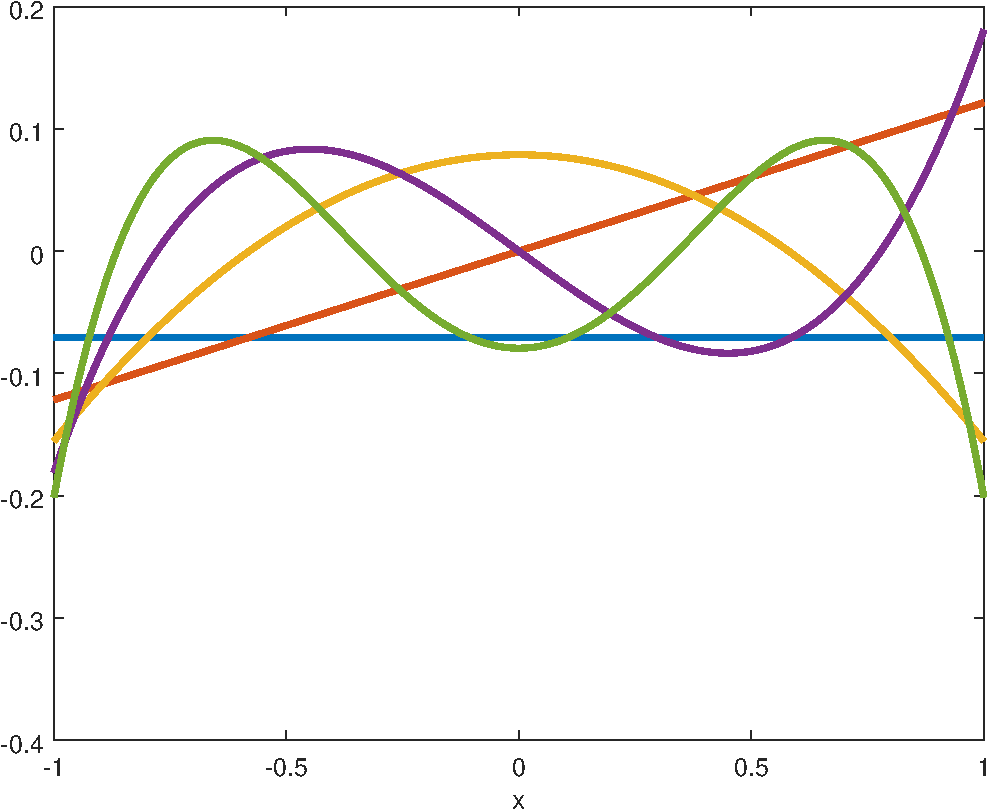
\includegraphics[width=0.55\textwidth]{figs/legendre} \quad 
\end{itemize}
\end{frame}


\end{document}

